\subsection{Развёртывание модулей и сервисов системы}
\label{sub:system-design:deployment}

Развертывание~-- процесс, сочетающий две взаимосвязанные концепции~-- процесса и архитектуры. Процесс развертывания заключается в доставке кода в промышленную среду и состоит из этапов, которые должны выполнить разработчики или системные администраторы.

Облачные вычисления~-- это способ предоставления системных ресурсов компьютера по требованию без активного участия пользователя в их управлении. Частные случаи таких ресурсов~-- хранилище данных (облачное) и вычислительные мощности. Облачные вычисления предоставляются потребителям в разных формах. Моделей обслуживания всего три основных, хотя в рамках конкретных бизнес-потребностей модели могут принимать подвиды. На рис.~\ref{fig:cloud-computing-service-models} представлены основные сервисные модели облачных вычислений. Все эти модели являются слоями над физическими вычислительными ресурсами, так модель \textit{SaaS} включает в себя все слои ниже, с той лишь разницей что для клиентов облака остальные слои скрыты и взаимодействие с ними происходит только лишь через слой \textit{SaaS}.

\begin{figure}[h]
\centering
    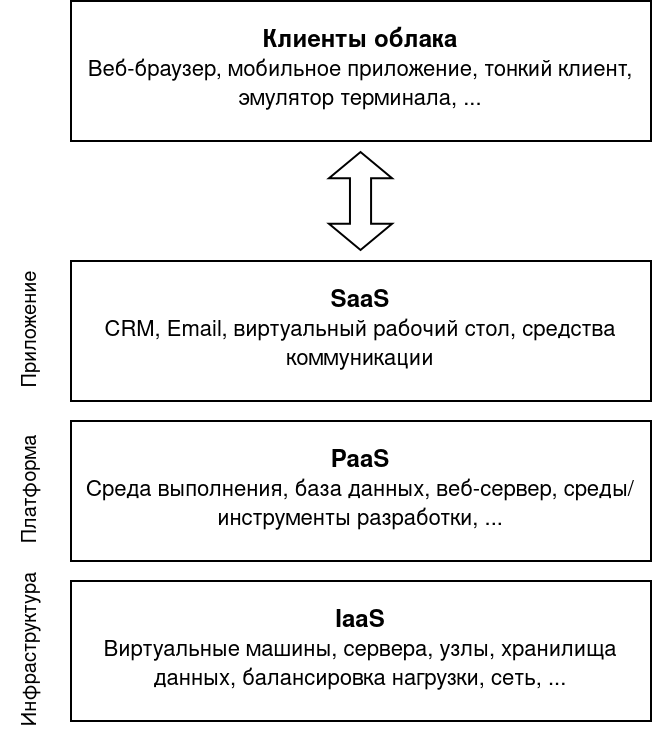
\includegraphics[width=0.5\linewidth]{assets/cloud-computing-service-models.png}
    \caption{Модели компьютерных вычислений в виде слоев}
    \label{fig:cloud-computing-service-models}
\end{figure}

\textit{Модель SaaS (Software as a Service)}~-- «Программное обеспечение как услуга»~-- модель, в которой потребителю предоставляется возможность использования прикладного программного обеспечения провайдера, работающего в облачной инфраструктуре и доступного из различных клиентских устройств или посредством клиента, например, из браузера (например, веб-почта) или посредством интерфейса программы.

\textit{Модель PaaS (Platform as a Service)}~-- «Платформа как услуга»~-- модель, когда потребителю предоставляется возможность использования облачной инфраструктуры для размещения базового программного обеспечения для последующего размещения на нём новых или существующих приложений (собственных, разработанных на заказ или приобретённых тиражируемых приложений). В состав таких платформ входят инструментальные средства создания, тестирования и выполнения прикладного программного обеспечения~-- системы управления базами данных, связующее программное обеспечение, среды исполнения языков программирования, предоставляемые облачным провайдером.

\textit{Модель IaaS (Infrastructure as a Service)}~-- «Инфраструктура как услуга» пре\-дос\-та\-вля\-ется как возможность использования облачной инфраструктуры для самостоятельного управления ресурсами обработки, хранения, сетями и другими фундаментальными вычислительными ресурсами, например, потребитель может устанавливать и запускать произвольное программное обеспечение, которое может включать в себя операционные системы, платформенное и прикладное программное обеспечение.

В рамках дипломного проекта в большей степени рассматривается модель \textit{PaaS}. Именно на этом слое разрабатываются микросервисы и формируется бизнес логика. Другими словами, именно на PaaS слое формируется слой выше (SaaS), который предоставляет уже конкретные услуги пользователям. Конкретными программными продуктами, реализующими модель PaaS, являются: \textit{Openshift}, \textit{Kubernetes}, \textit{Docker}, \textit{Docker Swarm}. Разработанный конечный продукт должен иметь возможность легко разворачиваться в любой из этих сред. Этого легко добиться, так как \textit{Openshift} платформа строится на \textit{Kubernetes}, а тот, в свою очередь, построен на основе \textit{Docker}. За счёт удачности решений эти программные продукты используются во многих компаниях и являются устоявшимся стандартом облачной разработки. Крупные провайдеры облачных платформ, такие как \textit{Amazon Web Services}, \textit{Google Cloud}, \textit{Microsoft Azure}, в том числе белорусский \textit{Hoster.by}, предоставляют возможность развернуть любой из приведенных выше продуктов.

С разработкой программного продукта необходимо разработать и схему процесса его автоматизированного развертывания в облаке, потому что конфигурация развертывания должна быть опубликована в \textit{PaaS}, чтобы процесс жизненного цикла приложения начался. Одной из особенностей облачных окружений является файл конфигурации развертывания~-- \textit{Deployment}, который непосредственно публикуется в среде \textit{PaaS}. В рамках дипломного проекта рассматривается \textit{PaaS} среда \textit{Kubernetes}~-- инструмент оркестрации \textit{Docker}, который обращается с набором серверов под управлением \textit{Docker}, как с пулом ресурсов. Архитектура фреймворка оркестрации \textit{Docker} представлена на рис.~\ref{fig:system-design:deployment:kubernetes-infrastructure}.

\begin{figure}[h]
\centering
    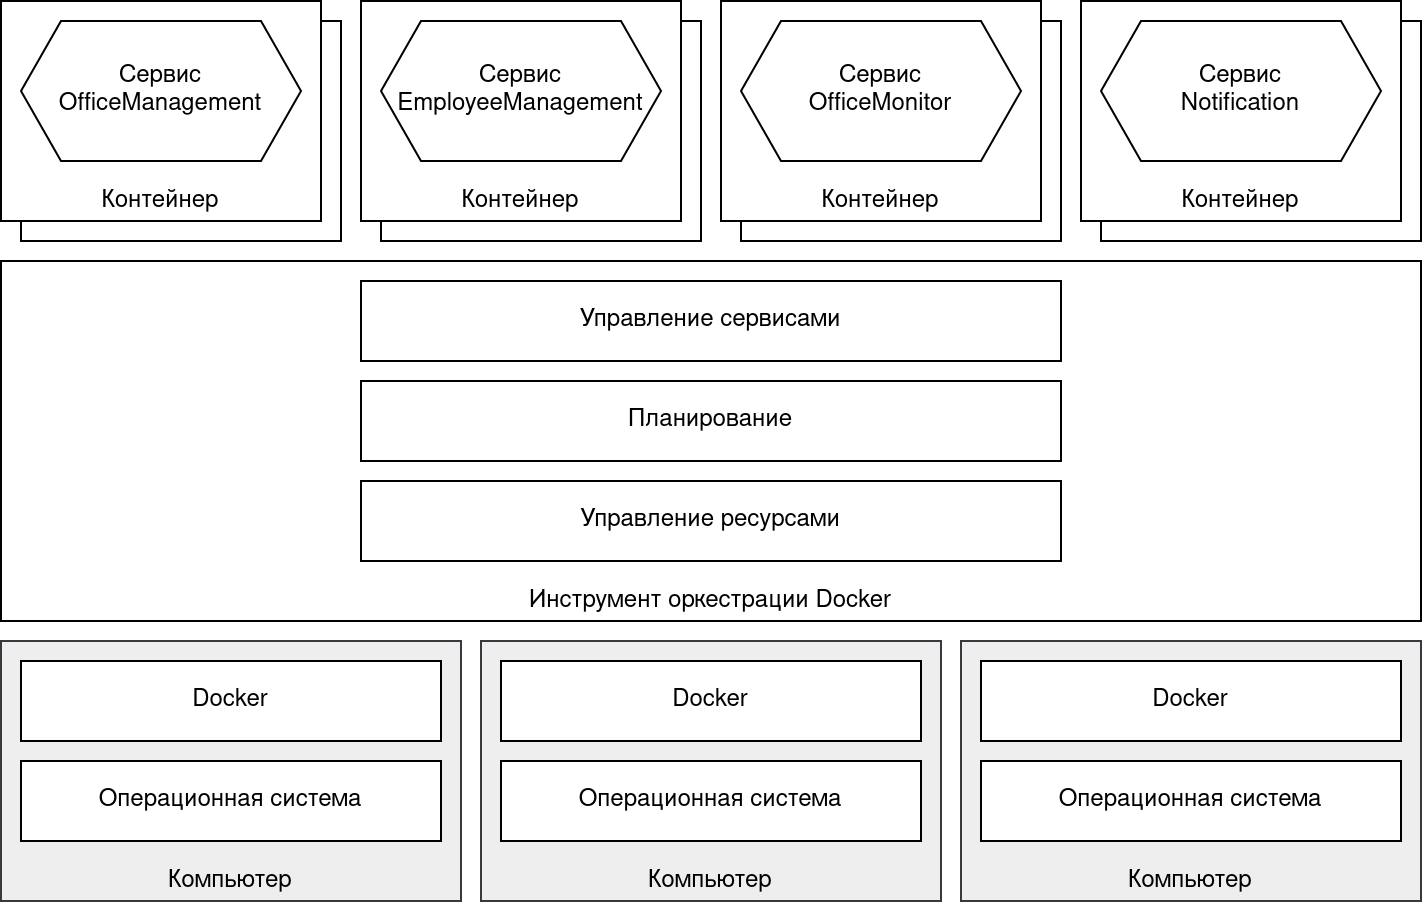
\includegraphics[width=0.99\linewidth]{assets/kubernetes-infrastructure.png}
    \caption{Архитектура \textit{Kubernetes}}
    \label{fig:system-design:deployment:kubernetes-infrastructure}
\end{figure}

Листинг конфигурации \textit{Deployment} \textit{Kubernetes} для развертывания микросервиса \textit{EmployeeManagement} приведен ниже:

\begin{lstlisting}[style=pythonstyle]
apiVersion: apps/v1
kind: Deployment
metadata:
  name: employee_management_service-backend-deployment
  namespace: office_management-production
spec:
  replicas: 2
  selector:
    matchLabels:
      type: backend
      service: employee_management
  strategy:
    type: RollingUpdate
    rollingUpdate:
      maxSurge: 1
      maxUnavailable: 1
  minReadySeconds: 10
  template:
    metadata:
      labels:
        type: backend
        service: employee_management
    spec:
      initContainers:
        - name: migrate
          image: employee_management_service-backend:latest
          envFrom:
            - secretRef:
                name: employee_management_service-backend-secrets
      containers:
        - name: backend
          image: employee_management_service-backend:latest
          envFrom:
            - secretRef:
                name: employee_management_service-backend-secrets
          ports:
            - containerPort: 8001
          resources:
            requests:
              memory: "512Mi"
              cpu: "250m"
            limits:
              memory: "1024Mi"
              cpu: "500m"
          readinessProbe:
            httpGet:
              path: /api/healthcheck
              port: 8001
            initialDelaySeconds: 10
          livenessProbe:
            httpGet:
              path: /api/healthcheck
              port: 8001
            initialDelaySeconds: 10
\end{lstlisting}

Важным пунктом конфигурации является свойство \textit{\lstinline!image!}, в нем указано имя образа контейнера, который будет браться из настроенного на хост машине репозитория \textit{Docker}-образов. Для большей наглядности изобразим полный путь контейнера от момента его создания (сборки) до момента попадания на хост машину с \textit{Kubernetes}. Свой жизненный путь \textit{Docker}-образ берет с исходного кода и \textit{Dockerfile}, где описано из чего создается образ, какие файлы, инструменты и программы он содержит в себе. Диаграмма состояния процесса сборки исходного кода микросервиса в \textit{Docker}-образ изображена на рис.~\ref{fig:docker-image-flow}.

\begin{figure}[h]
\centering
    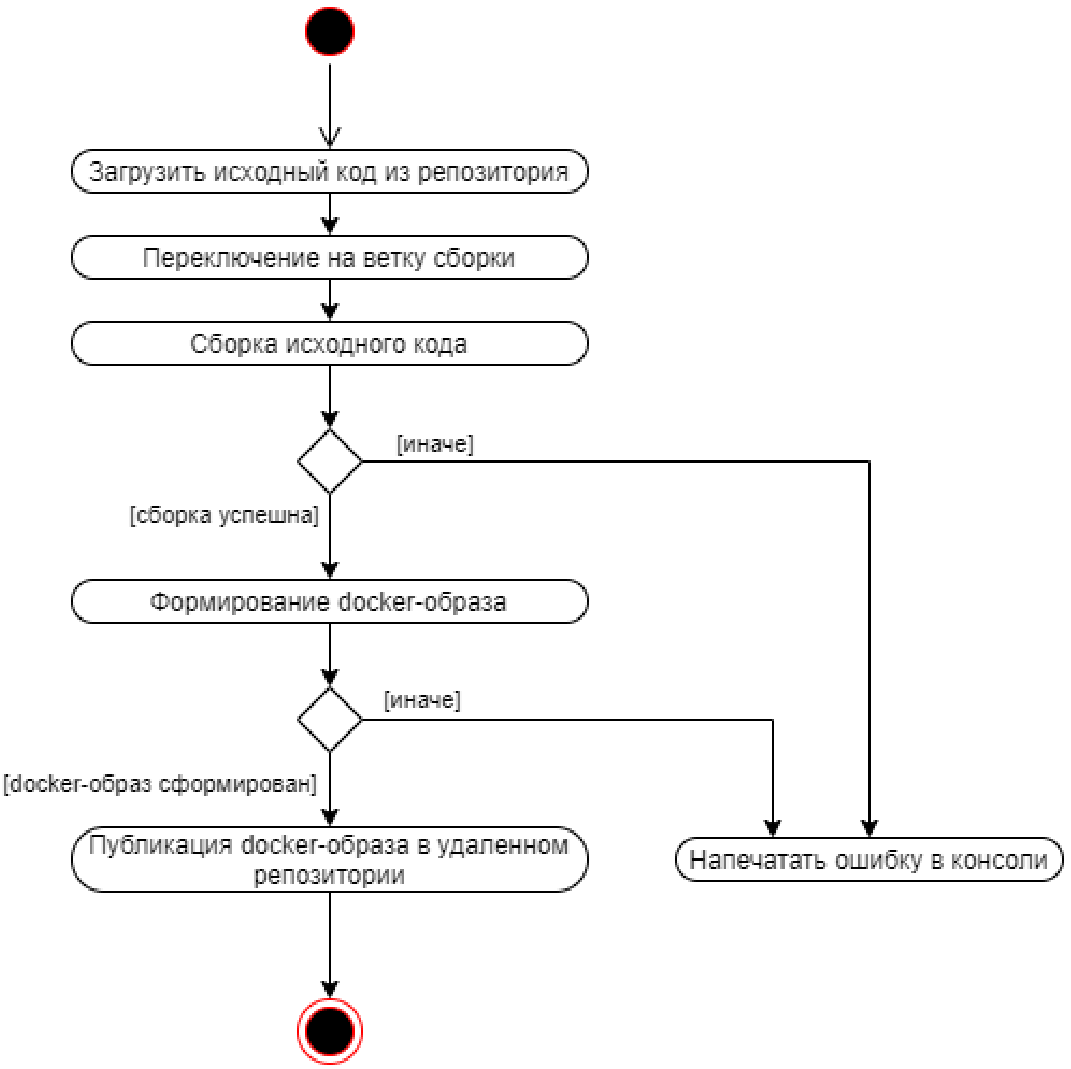
\includegraphics[width=0.75\linewidth]{assets/docker-image-flow.png}
    \caption{Диаграмма состояния процесса сборки исходного кода микросервиса в \textit{Docker}-образ}
    \label{fig:docker-image-flow}
\end{figure}

Рассмотрим концептуальную схему работы программного средства. Клиенты взаимодействуют с сервисами, предназначенными для сокрытия набора \textit{Pod} под одним \textit{DNS} именем. Например, возможен вариант реализации нескольких экземпляров \textit{API-Gateway} запущенных в облаке, однако обращение к ним возможно через \textit{DNS} имя \textit{\lstinline!api-gateway!}. Таким образом, \textit{Service} в \textit{Kubernetes}~-- это \textit{DNS} запись, скрывающая несколько \textit{IP}-адресов запущенных экземпляров приложения~\cite{book_production_kubernetes}. Набор \textit{Pod}-экземпляров является олицетворением запущенных \textit{Docker} контейнеров. Жизненный цикл \textit{Pod} определяется ресурсом \textit{Deployment}, рассмотренным ранее. Фигурой документа изображены самописные ресурсы, опубликованные в облаке, которые создаются и описываются разработчиком.

Под клиентом подразумевается либо человек, либо другой микросервис, который использует опубликованное \textit{API}. Взаимодействие с сервисами выражено путем отправки \textit{HTTP}-запросов к \textit{API-Gateway}, который при наличии соответствующего правила маршрутизации перенаправит запрос к целевому микросервису. На рисунке~\ref{fig:kubernetes-conceptual-architecture} представлена облачная среда под управлением \textit{PaaS} \textit{Kubernetes}. Все фигуры, кроме клиентов обозначают серверные облачные ресурсы. 

\begin{figure}[h]
\centering
    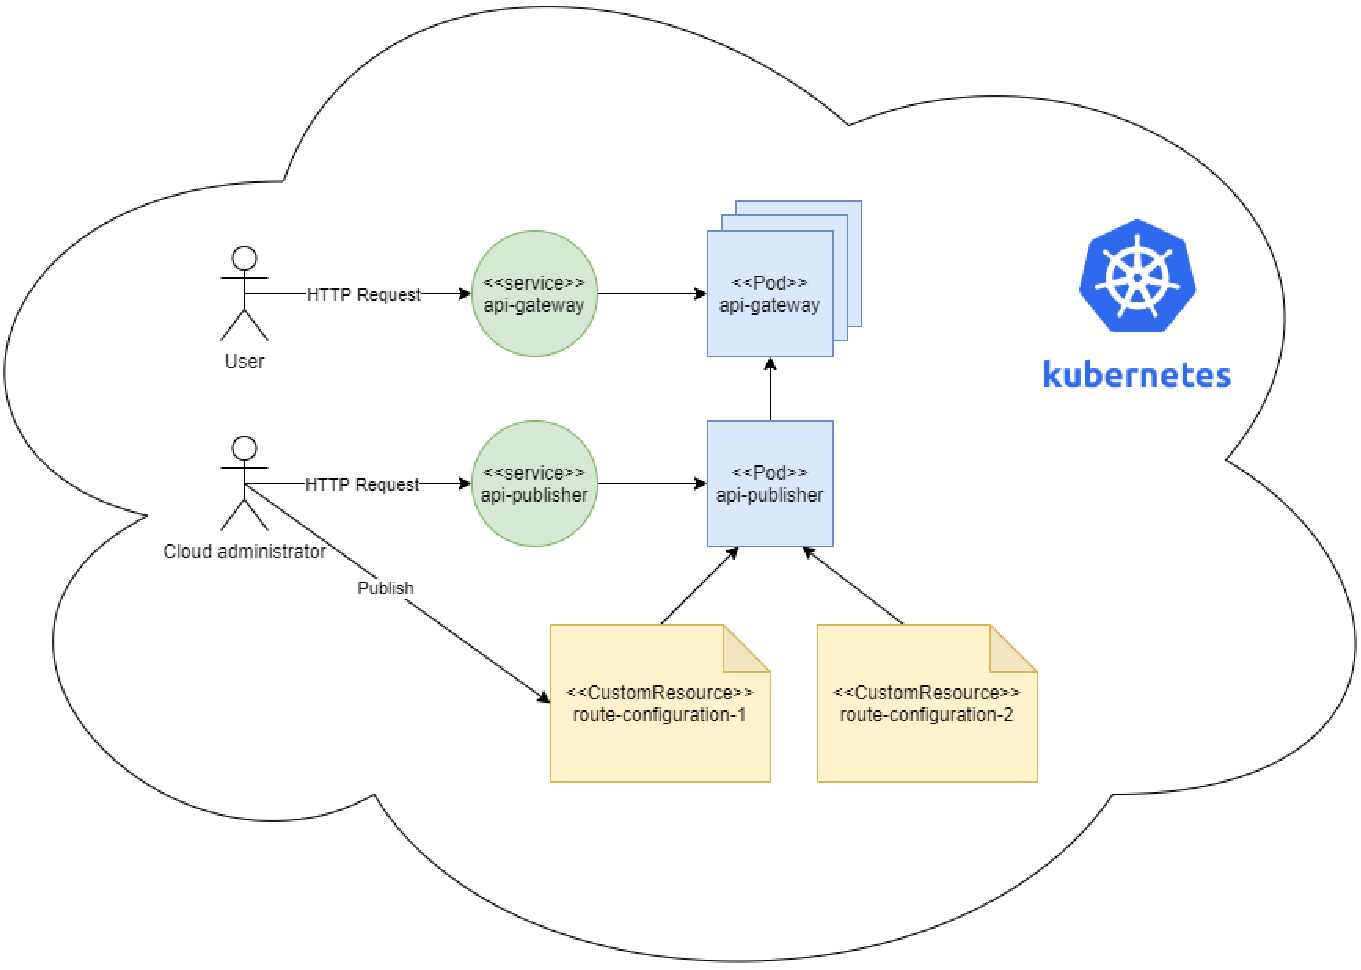
\includegraphics[width=0.8\linewidth]{assets/kubernetes-conceptual-architecture.png}
    \caption{Концептуальная архитектура \textit{PaaS} \textit{Kubernetes}}
    \label{fig:kubernetes-conceptual-architecture}
\end{figure}
